\chapter{Konzeption und Realisierung}
\label{ch:04_konzeption_realisierung}

Im folgenden Kapitel wird der Aufbau und die technische Umsetzung des in C++ und OpenGL
implementierten Test-Frameworks \ac{HyDra} beschrieben.
Es werden die Struktur der Daten, die Implementierungen der untersuchten Rendering-Pipelines, die Implementierungen der
verwendeten \ac{NPR}-Effekte, die individuellen architektonischen Limitationen sowie die Umsetzung der
Leistungsmessungskomponenten erläutert.
Das implementierte Programm fungiert als Untersuchungs- und Messinstrument, das eine Sandbox-Umgebung bereitstellt, in
der das Verhalten der verschiedenen Rendering-Pipelines erprobt werden kann.

Der Aufbau des \ac{HyDra} Frameworks folgt im Wesentlichen den Kernparadigmen der maximalen Vergleichbarkeit und des
Determinismus.
Das Programm wurde so strukturiert, dass die drei Rendering-Pipelines unter identischen Bedingungen getestet werden
können.


\section{Systemarchitektur und Lebenszyklus}
\label{sec:0401_system_architecture_and_lifecycle}

Die Architektur des \ac{HyDra}-Frameworks ist durch die Entkopplung der logischen Szenenverwaltung (\ac{CPU}-Zustand)
vom eigentlichen Rendering (\ac{GPU}-Dispatch) gekennzeichnet.
Es wird garantiert, dass alle drei Rendering-Pipelines exakt denselben deterministischen Zustand als Eingabedaten
erhalten.
Ziel ist es, etwaigen individuellen \ac{CPU}-Overhead möglichst zu eliminieren.
Für die Deferred-Pipelines wird zudem der Semantische G-Buffer aufbereitet, wofür im Rahmen der Szeneverwaltung
zusätzlich die Vergabe von objektspezifischen \textit{Style-IDs} erfolgt.
Ein weiterer Bestandteil dieser vorbereitenden \ac{CPU}-Logik ist das implementierte View-Frustum-Culling.
Es fungiert als Filter, der die sichtbare Geometrie evaluiert, bevor die Grafikkarte involviert wird.

\subsection{Frame-Lebenszyklus}
\label{subsec:040101_frame_lifecycle}

% Init
Wie in Abbildung~\ref{fig:render_loop_swimlane} dargestellt, durchläuft das Framework vor dem Eintritt in die
Haupt-Rendering-Schleife ein initiales Setup.
Diese Phase erfüllt im Wesentlichen zwei architektonische Aufgaben: Zum einen die Speicherallokation (\ac{VRAM}) der
benötigten \ac{FBO}s, des \ac{G-Buffer}s sowie der \ac{VAO}s und \ac{VBO}s.
Zum Anderen das Laden, Kompilieren und Verlinken aller Shader-Programme inklusive des Uniform-Mappings.
Die in dieser einmaligen Initialisierungsphase definierte Basiskonfiguration kann zur Laufzeit partiell rekonfiguriert
werden (etwa durch dynamische Skalierung der Auflösung oder Anpassung der Bitrate der \ac{G-Buffer}-\ac{FBO}s).
Der Kontrollfluss wird erst an die zyklische Ausführung des Main-Loops übergeben, wenn der initiale Aufbau des \ac{VRAM}
und der Render-Pipelines vollständig abgeschlossen ist.

% Sync.
Am Anfang der Haupt-Rendering-Schleife werden die für die spätere Hardware-Performance-Evaluation relevanten Timer
initialisiert.
Gleichzeitig wird eine explizite Limitierung der Frame-Taktung (\texttt{AwaitCapacity()}) erzwungen, um zu verhindern,
dass die \ac{CPU} der asynchronen \ac{GPU}-Abarbeitung zeitlich zu weit vorausläuft.
Ein derartiger Rückstand der Grafikkarte würde die Latenz- und Profiler-Messungen andernfalls systematisch verfälschen.

% Input.
Im direkten Anschluss steuert ein dezidiertes \texttt{InputController}-Modul die Modifikation des Szenenzustands.
Diese Komponente ermöglicht eine manuelle Interaktion zur Laufzeit, um spezifische Performance-Metriken, visuelle
Artefakte oder systemische Limitierungen der einzelnen Pipelines interaktiv untersuchen zu können.

% Culling & Upload.
Vor der eigentlichen Datenübertragung an die \ac{GPU} wird die Geometrie einem \ac{CPU}-seitigen logischen Pass
unterzogen.
Ein \textit{View-Frustum-Culling} dient hierbei als Filter, um Geometrien, die sich außerhalb des
sichtbaren Bereichs der Kamera befinden, von der weiteren Verarbeitung auszuschließen.
Für die verbleibenden, sichtbaren Entitäten erfolgt anschließend der \ac{PCIe}-Speichertransfer
(\texttt{rlUpdateVertexBuffer()}) der Modell-Transformationsmatrizen und Style-IDs.

% Dispatch.
Nachdem die Datenpräparation auf der \ac{CPU} abgeschlossen ist, wird die Ausführung der selektierten Rendering-Pipeline
orchestriert.
In dieser Phase (\textit{Render Dispatch}) werden die notwendigen Zustandsänderungen der \ac{API} vorgenommen und die
instanziierten Draw-Calls an die \ac{GPU} übermittelt.
Die Grafikhardware übernimmt daraufhin, asynchron zum Main-Thread, die Rasterisierung und Ausführung der definierten
Shader-Logik.
Die exakte Implementierung der Rendering-Pipelines wird in den nachfolgenden Kapiteln evaluiert.

% Telemetry Drain.
Den Abschluss eines Frame-Zyklus bildet die Präsentation des finalen Bildes auf dem Bildschirm.
Zusätzlich werden die asynchronen Hardware-Timer der \ac{GPU} ausgelesen (\texttt{QueryOldestResult()}).
Dieser \textit{Drain}-Prozess erfolgt explizit nicht-blockierend, um die fortlaufende Ausführung der \ac{GPU} für
nachfolgende Messungen nicht durch künstliche \ac{CPU}-Stalls zu unterbrechen.
Hierdurch wird gewährleistet, dass der tatsächliche Render-Overhead der Pipelines isoliert quantifizierbar bleibt.

% Ablaufdiagramm: Frame Lebenszyklus
\begin{figure}[htbp]
    \centering
    \resizebox{\textwidth}{!}{%
        \begin{tikzpicture}[
            >=Latex,
            font=\sffamily,
        % Styles für UML-Elemente
            activity/.style={rectangle, draw=black, thick, rounded corners, inner sep=6pt, minimum width=4.8cm,
            align=center, fill=white},
            crosslane/.style={rectangle, draw=black, thick, rounded corners, inner sep=6pt, minimum width=5.0cm,
            align=center, fill=gray!10},
            branchact/.style={rectangle, draw=black, thick, rounded corners, inner sep=6pt, minimum width=3.0cm,
            minimum height=1.2cm, text width=3.0cm, align=center, fill=white},
            hwblock/.style={rectangle, draw=black, thick, rounded corners, inner sep=8pt, minimum width=6.0cm,
            align=center, fill=gray!20},
            end/.style={circle, draw=black, fill=white, minimum size=0.5cm, double=black, double distance=1.5pt},
            edge/.style={->, thick, rounded corners=3pt},
            dataedge/.style={->, thick, dashed, draw=blue!80!black, rounded corners=3pt}
        ]
            % Hintergrund
            \draw[thick, dotted, gray] (-3.5, 3.0) -- (16.0, 3.0);
            \node[anchor=south west, text=gray, font=\sffamily\bfseries] at (-3.5, 3.1) {Engine Initialisierung};

            \draw[thick, dotted, gray] (-3.5, 0.2) -- (16.0, 0.2);
            \node[anchor=south west, text=gray, font=\sffamily\bfseries] at (9.0, 0.3) {CPU-Logik \&
            Haupt-Render-Schleife};

            \draw[thick, dotted, gray] (-3.5, -8.7) -- (16.0, -8.7);
            \node[anchor=south west, text=gray, font=\sffamily\bfseries] at (-3.5, -8.6) {GPU Pipeline Ausführung};

            \draw[thick, dotted, gray] (-3.5, -17.2) -- (16.0, -17.2);
            \node[anchor=south west, text=gray, font=\sffamily\bfseries] at (-3.5, -17.1) {Abschluss \& Telemetrie};

            % Swimlanes und Header
            \draw[thick, loosely dashed, gray] (7.0, 4.5) -- (7.0, -21.0);
            \node[font=\bfseries\large, anchor=south] at (2.5, 3.8) {CPU};
            \node[font=\bfseries\large, anchor=south] at (11.5, 3.8) {GPU};


            % Knoten Definitionen
            % Phase 1
            \node[activity] (init) at (2.5, 1.8) {Engine Setup \\ \texttt{RenderContext::Init()} \\
            {\scriptsize (Shader \& FBO Allokation)}};
            \node[activity] (sync) at (2.5, -1.2) {Zeitmessung \& Limitierung \\ \texttt{AwaitCapacity()} \\
            {\scriptsize (Blockiert bei GPU-Rückstand)}};
            \node[activity] (input) at (2.5, -3.2) {State-Injektion \\ \texttt{InputController}};
            \node[activity] (culling) at (2.5, -5.2) {Logischer Szenen-Pass \\ \texttt{UpdateVisibility()} \\
            {\scriptsize (Frustum-Culling \& Licht)}};
            \node[crosslane] (upload) at (7.0, -7.2) {VBO Speicher-Transfer (PCIe) \\ \texttt{rlUpdateVertexBuffer()} \\
            {\scriptsize (Szene-Objekte inkl. Style-IDs)}};
            \node[activity] (dispatch) at (2.5, -9.7) {Render Dispatch \\ {\scriptsize (GPU-Kommandos absetzen)}};
            \node[diamond, aspect=2.5, draw=black, thick, align=center, fill=white, inner sep=1pt] (routing) at
            (11.5, -10.7) {Render-Pfad?};
            \node[branchact] (fwd) at (8.3, -12.7) {Forward \\ Pipeline};
            \node[branchact] (uber) at (11.5, -12.7) {Deferred-Uber \\ Pipeline};
            \node[branchact] (vol) at (14.7, -12.7) {Deferred-Volume \\ Pipeline};
            \coordinate (merge_point) at (11.5, -14.2);
            \node[hwblock] (gpu_render) at (11.5, -15.7) {\textbf{Asynchrone Ausführung der Grafikpipelines} \\
            {\scriptsize (Rasterisierung, G-Buffer \& Shader)}};
            \node[activity] (present) at (11.5, -18.7) {Ausgabe des fertigen Frames \\ auf dem Bildschirm};
            \node[activity] (drain) at (2.5, -18.7) {Telemetrie Drain \\ \texttt{QueryOldestResult()}};

            % Kontrollfluss
            \draw[edge] (init) -- (sync);
            \draw[edge] (sync) -- (input);
            \draw[edge] (input) -- (culling);
            \draw[edge] (culling.south) |- (upload.west);
            \draw[edge] (upload.south) |- (dispatch.east);
            \draw[edge] (dispatch.south) -- (drain.north);
            \draw[edge] (drain.south) -- ++(0, -0.4) -| (-4.0, -1.2) -- (sync.west) node[pos=0.25, above=2pt,
            font=\scriptsize\bfseries] {Nächster Frame};
            \draw[edge] (routing.west) -| (fwd.north);
            \draw[edge] (routing.south) -- (uber.north);
            \draw[edge] (routing.east) -| (vol.north);
            \draw[thick] (fwd.south) |- (merge_point);
            \draw[thick] (vol.south) |- (merge_point);
            \draw[thick] (uber.south) -- (merge_point);
            \draw[edge] (merge_point) -- (gpu_render.north);
            \draw[edge] (gpu_render.south) -- (present.north);

            % Datenfluss
            \draw[dataedge] (dispatch.east) -| (routing.north) node[pos=0.25, above=2pt, font=\scriptsize]
                {Push Commands};
            \draw[dataedge] (gpu_render.west) -- (7.0, -15.7) -- (7.0, -18.7) -- (drain.east) node[midway, below=2pt,
            font=\scriptsize] {Timer (bereit)};

        \end{tikzpicture}%
    }
    \caption[UML-Aktivitätsdiagramm des Frame-Lebenszyklus]{UML-Aktivitätsdiagramm des Frame-Lebenszyklus innerhalb des
    HyDra-Frameworks.}
    \label{fig:render_loop_swimlane}
\end{figure}

\subsection{Szeneverwaltung}
\label{subsec:040102_scene_management}

% Einleitung.
Die inhaltliche Verwaltung der dargestellten Szene wird im \ac{HyDra}-Framework von einem dedizierten
Szenenmanager-Modul (\texttt{SceneManager}) übernommen.
Dieses verwaltet den deterministischen Aufbau der Geometrie, insbesondere die Punktlicht-Proxies und die beleuchteten
Geometrien.
Die Geometrien werden prozedural mithilfe eines festgelegten Seeds erstellt.
Es wird sichergestellt, dass jeder Programmaufruf oder jede Änderung durch den Input-Controller zu vollständiger
Szeneparität hinsichtlich der Geometrieverteilung unter den gegebenen Parametern Objektanzahl, Punktlichtanzahl,
Lichtintensität und Objektdichte (Radius des Objektclusters) führt.
Die Szeneparität zwischen Aufrufen und bei Laufzeit-Manipulationen ist während der Performancemessungen hinsichtlich der
untersuchten (Stil-)Entropie, beispielsweise bezüglich der Style-ID-Verteilung oder Geometrieüberlappungen, von
besonders großer Wichtigkeit.

% Datenhaltung.
Die Datenhaltung der Szenegeometrien und Punktlicht-Proxies mitsamt ihrer assoziierten Style-IDs und
Transformationsmatrizen erfolgt in Arrays, die mit der Maximalanzahl der erstellbaren Objekte vorallokiert wurden.
Jeder Geometrie wird ein Index zugewiesen, anhand dessen für jedes Objekt drei Arrays für die Style-ID, die räumliche
Position und die bereits vorab berechnete Transformationsmatrix gespeichert werden
(\ac{SoA}-Muster)~\cite[S.~793]{akenine-mollerRealtimeRendering2019}.

% Entropie.
Hervorzuheben ist hier die Logik bezüglich der Stilentropie-Steuerung, die zwischen gestreuten (hohe Entropie) und
geordneten (niedrige Entropie) Verteilungen wechselt.
Die Zuweisung der Stil-ID erfolgt in Listing ~\ref{lst:style_assignment} und beschreibt die Gruppierung/Sortierung
innerhalb des \ac{HyDra}-Frameworks in der kreisförmigen Objektwolke mit anteiliger Aufteilung der Stile.

% Entropie Listing.
\begin{listing}[htbp]
    \begin{codeframe}
        \begin{minted}{cpp}
float styleId;
if (state.useClusteredStyles) {
    float normAngle = std::fmod(angle, 2.0f * PI);
    if (normAngle < 0.0f)
        normAngle += 2.0f * PI;
    // Divide the 2PI circle by the current number of active styles
    const float slice = (2.0f * PI) / numStyles;
    const int clusterIndex =
        std::clamp(static_cast<int>(normAngle / slice), 0, static_cast<int>(numStyles - 1));
    styleId = activeStyles[clusterIndex];
} else {
    // Distribute using the current pool size
    styleId = activeStyles[i % static_cast<int>(numStyles)];
}
        \end{minted}
    \end{codeframe}
    \caption{C++ Code zur Berechnung der \texttt{styleId}-Verteilung basierend auf dem Cluster-Status in
    HyDra-Framework.}
    \label{lst:style_assignment}
\end{listing}

% Culling-Mechanismus.
Die Prüfung der Sichtbarkeit erfolgt mittels eines klassischen Schnitttests der Bounding-Spheres gegen die sechs Ebenen
des Kamera-View-Frustums~\cite[S.~688, Abschn. \textit{Frustum Culling}]{gregoryGameEngineArchitecture2018}.
Darüber hinaus wird die Größe (der Radius) der Light-Volume-Proxies für die Deferred-Volume-Pipeline durch die
Lichtintensität beeinflusst~\cite[S.~891]{akenine-mollerRealtimeRendering2019}.
Im Rahmen des View-Frustum-Cullings werden diese ebenfalls berücksichtigt, um die Darstellung von Lichtern, deren
Wirkungsbereich vollständig außerhalb des Sichtfeldes liegt, zu vermeiden und somit keine unnötigen
Beleuchtungsberechnungen für spätere Performance-Evaluationen zu verursachen.

% Forward Unterschied.
Das Resultat des Szeneaufbaus ist abhängig von der gewählten Rendering-Pipeline.
Während die Deferred-Pipelines die sichtbaren Instanzen als zusammenhängende, lineare Arrays für den Upload erhalten,
erzwingt das Forward-Rendering eine Aufspaltung der Daten.
Der SceneManager durchläuft hierfür eine Iteration über die Style-IDs der sichtbaren Objekte und ordnet diese in
pipelinespezifische Queues (z.\ B.\ \texttt{fwdTransformsGooch}, \texttt{fwdTransformsToon}) an.
Dieser Sortiervorgang auf der \ac{CPU} ist eine architektonische Notwendigkeit des Forward-Ansatzes, um
kostenintensive Shader-State-Changes auf der \ac{GPU} zu
bündeln~\cite[S.~795 u. S.~886]{akenine-mollerRealtimeRendering2019}.

\subsection{Datenfluss der Stilisierung und G-Buffer Layout}
\label{subsec:040103_g-buffer_layout}

% Style-Id Datenfluss.
Für jedes Objekt werden Style-IDs definiert, die die verschiedenen verwendeten Shading-Effekte referenzieren.
Die Definition dieser Style-IDs erfolgt über dynamische Vertex-Buffer (\ac{VAO}s und \ac{VBO}).
Schließlich werden die Style-IDs als instanziierte Vertex-Attribute für jede Geometrie in den Vertex-Shader
übertragen.
Die Style-IDs werden nicht pro Vertex, sondern einmal pro Instanz im Vertex-Shader ausgelesen, um sie
effizient an den Fragment-Shader weiterzureichen, der die \ac{G-Buffer}Textur
erstellt~\cite[S.~797-798]{akenine-mollerRealtimeRendering2019}.
In der Forward Pipeline erfolgt die Mitlieferung der Style-IDs pro verarbeiteter Geometrie direkt in den
Shader-Aufrufen (Draw-Calls).

% G-buffer Layout.
Wie in Tabelle~\ref{tab:gbuffer_layout} aufgezeigt wird für das \texttt{\ac{RT}0} (Albedo) ein 8-Bit-Format
(\texttt{R8G8B8A8}) genutzt.
Für den Normalen-Puffer (\texttt{\ac{RT}1}) wird hingegen ein 16-Bit-Format \texttt{R16G16B16A16} verwendet.
Diese erhöhte Präzision ist eine architektonische Notwendigkeit, da geringere Bittiefen bei den nachfolgenden
Screen-Space-Lichtberechnungen unzureichend sind~\cite[Folie~37]{AdvancesRealTimeRendering}.
Die genauen visuellen Auswirkungen (Banding-Artefakte), die diesen Kompromiss zugunsten einer höheren Speicherbandbreite
erzwingen, werden in der Evaluation der Deferred-Volume-Pipeline in Kapitel~\ref{subsec:040203_deferred_volume_pipeline}
im Detail dargelegt.

\begin{table}[htbp]
    \caption{Spezifikation des G-Buffer-Layouts im \ac{HyDra}-Framework.}
    \label{tab:gbuffer_layout}
    \centering
    \small
    \renewcommand{\arraystretch}{1.3}
    \begin{tabularx}{\textwidth}{l | l X X X X}
        \hline
        \textbf{Render Target} & \textbf{Format} & \textbf{Kanal R} & \textbf{Kanal G} & \textbf{Kanal B} &
        \textbf{Alpha} \\
        \hline
        \textit{RT0 (Albedo)}  & \texttt{R8G8B8A8}        & \texttt{BaseColor R}    & \texttt{BaseColor G}
        & \texttt{BaseColor B}    & \texttt{BaseColor A}    \\

        \hline

        \textit{RT1 (Normal)}  & \texttt{R16G16B16A16}    & \texttt{World Normal X} & \texttt{World Normal Y}
        & \texttt{World Normal Z} & \textbf{Style-ID}       \\

        \hline

        \textit{Depth}         & \texttt{8-Bit Grayscale} & \texttt{Linear Depth}   & \texttt{--}
        & \texttt{--}             & \texttt{--}             \\
        \hline
    \end{tabularx}
\end{table}

% Die Style-ID.
Der semantische Kern der hybriden Stilisierung liegt in der Persistierung der durchgereichten Instanz-Metadaten.
Wie in Tabelle ~\ref{tab:gbuffer_layout} ersichtlich, wird die komprimierte Style-ID in den ungenutzten Alpha-Kanal des
Normalen-\ac{RT} encodiert.
Durch dieses Mapping stehen den nachgelagerten Deferred-Shadern sämtliche benötigten Metadaten pro Fragment zur
Verfügung und die \ac{GPU} kann im Shading dynamisch und selektiv den korrekten \ac{NPR}-Algorithmus auswählen.


\section{Pipeline-Architekturen und systematische Restriktionen}
\label{sec:0402_pipelines_and_restrictions}

% Einordnung
In Kapitel~\ref{ch:02_grundlagen}, wurden die theoretischen Paradigmen der grundlegenden Rendering-Pipelines
etabliert.
In diesem Abschnitt werden die tatsächlichen architektonischen Restriktionen der implementierten Renderpfade innerhalb
des \ac{HyDra}-Frameworks analysiert.
Der Fokus liegt demnach nicht auf der grundlegenden Funktionsweise, sondern auf den spezifischen Modifikationen zur
Integration selektiver Stilisierungsprozesse und den daraus resultierenden Hardware-Limitationen.
Im Rahmen der vorliegenden Untersuchung erfolgt eine Analyse der absoluten Skalierungsgrenzen (Bottlenecks) und
spezifischen visuellen Artefakte (Drawbacks) der jeweiligen Architekturen, um das theoretische Fundament für die
quantitative Performance-Evaluation in Kapitel~\ref{ch:05_evaluation} zu legen.

\subsection{Forward Rendering Pipeline}
\label{subsec:040201_forward_pipeline}

% Grundlagen der Verarbeitung.
Die Umsetzung der Forward-Pipeline innerhalb des \ac{HyDra}-Frameworks folgt der klassischen
Standardimplementierung, wie in Kapitel~\ref{ForwardExplanation} dargelegt und stellt eine vergleichende
\textquote{Baseline} dar.
Die Forward-Pipeline wird entsprechend ohne zusätzliche Optimierungen wie einen Z-Prepass oder anderweitige Variationen
implementiert.

% Stilisierung.
Wie in Kapitel~\ref{subsec:040102_scene_management} dargelegt, erfolgt die selektive Stilisierung in der
Forward-Pipeline unmittelbar während der Drawcalls der in Batches instanziierten und von der \ac{CPU}
(dem \texttt{SceneManager}) aufbereiteten Geometrie-Arrays.
Demzufolge wird jedem Objekt der entsprechende Fragment-Shader sowie der damit assoziierte \ac{NPR}-Stil direkt
zugewiesen.

% Uniform Limits.
Dieser Ansatz weist, vor allem in Hinblick auf die selektive Stilisierung, allerdings diverse Schwachstellen und
Limitationen auf.
Eine wesentliche Schwachstelle ist die Begrenzung in Form von vorherrschenden Uniform-Buffer-Limits.
In der für das Framework gewählten Grafik-\ac{API} OpenGL 3.3 erfolgt die Übergabe der Lichtdaten-Arrays standardmäßig über
\ac{UBO}s, um den \ac{CPU}-seitigen Overhead einzelner Uniform-Zuweisungen pro Lichtquelle zu
minimieren~\cite[S.~798]{akenine-mollerRealtimeRendering2019}.
Die maximale physische Speichergröße, die ein einzelner Uniform-Block umfassen darf, wird treiberseitig durch das
hardwareabhängige Limit \texttt{GL\_MAX\_UNIFORM\_BLOCK\_SIZE} definiert.
Während dieser Wert auf moderner Desktop-Hardware variiert, schreibt die OpenGL-3.3-Spezifikation herstellerübergreifend
eine garantierte Mindestgröße von \texttt{16 KiB} vor~\cite[S.~321, Tab.~6.45]{OpenGL33Core2010}.

Wird jede der Punktlichtquellen im Shader durch eine vereinfachte Struktur aus einer Positions- und einer
Farb-/Intensitätskomponente mit einer Gesamtgröße von \texttt{32 Bytes} abgebildet, lässt sich die theoretisch maximale
Lichtanzahl $N_{\text{Licht}}$ innerhalb des garantierten \ac{API}-Mindestlimits über folgende Relation bestimmen:
\begin{equation}
    N_{\text{Licht}} = \frac{\texttt{GL\_MAX\_UNIFORM\_BLOCK\_SIZE}}{\text{Größe pro Lichtquelle}} =
    \frac{16.384\text{ Bytes}}{32\text{ Bytes}} = 512
    \label{eq:ubo-limits}
\end{equation}

Auf Hardware-Ebene existiert diese Restriktion, weil Uniform-Daten in dedizierten, extrem schnellen On-Chip-Registern
(Constant Registers) der \ac{GPU} gehalten werden müssen~\cite[S.~35]{akenine-mollerRealtimeRendering2019}.
Dieses fundamentale \ac{API}-Limit begründet, warum die Single-Pass-Architekturen des Frameworks
(Forward und Deferred-Uber) auf eine Kapazitätsgrenze von maximal 500 Punktlichtern beschränkt sind, um eine vollständige
Plattformkompatibilität ohne Treiber-Abstürze zu gewährleisten.

% Screen Space Limits.
Eine weitere grundlegende Einschränkung der naiven Forward-Pipeline bezüglich selektiver Stilisierung ist, dass sich
traditionelle Screen-Space- oder Post-Processing-Effekte wie ein Kuwahara-Filter oder Sobel-Outlines nicht selektiv bzw.
partiell anwenden lassen.
Für die Generierung dieser Effekte ist präzises Wissen bezüglich der finalen Szene sowie der Umgebungsgeometrie
erforderlich~\cite[Abschn.~5]{magdicsPostprocessingNPREffects2013}.
Im Rahmen des implementierten Forward-Renderings erfolgt die Anwendung der Shader direkt und isoliert auf die einzelnen
Geometrien innerhalb der Draw-Calls, wodurch keine Umgebungsbezogenen Daten (semantische Objektidentität) des finalen
Bildes während des Shadings auf der \ac{GPU} vorhanden sind.
Eine selektive Realisierung solcher Effekte ist in naiven Single-Pass Forward-Pipelines also nicht möglich.
In Bezug auf den im \ac{HyDra}-Framework implementierten Effekt zur Darstellung von Konturen kann in der
Forward-Pipeline, anstelle der in den Deferred-Pipelines verwendeten Sobel-Outlines (Screen-Space-Methode) das bedingt
gleichwertige Inverted-Hull-Verfahren (Object-Space-Methode) zur Kantenzeichnung verwendet werden
(siehe Abbildung~\ref{fig:040201_outline_comparison}).
Diese nur äußerst bedingte visuelle Parität muss für etwaige vergleichende Evaluationen berücksichtigt werden.

% Abbildung aus Engine.
\begin{figure}[htbp]
    \centering
    % Linkes Bild
    \begin{subfigure}[b]{0.49\textwidth}
        \centering
        
\includegraphics[width=0.85\linewidth]{abbildungen/hydra_capture_20260713_083726}
        \caption{Inverted-Hull + Toon-Shading in Forward}
        \label{fig:hydra_inverted-hull}
    \end{subfigure}
    \hfill
    % Rechtes Bild
    \begin{subfigure}[b]{0.49\textwidth}
        \centering
        
\includegraphics[width=0.85\linewidth]{abbildungen/hydra_capture_20260713_083735}
        \caption{Sobel-Outlines + Toon-Shading in Deferred}
        \label{fig:hydra_sobel-outlines}
    \end{subfigure}
    \caption{Toon-Shading und Vergleich von Kontureffekten in Forward- und Deferred-Pipelines mittels Inverted-Hull- und
    Sobel-Outline-Verfahren in HyDra-Framework.}
    \label{fig:040201_outline_comparison}
\end{figure}

\subsection{Deferred-Uber Rendering Pipeline}
\label{subsec:040201_deferred_uber_pipeline}

% Einleitung und Aufbau
Im \ac{HyDra}-Framework wird zur Referenz eines einfachen Deferred-Ansatzes eine Deferred-Pipeline in einer
Single-Pass-Architektur (bezogen auf den Lighting-Pass) mittels Uber-Shader-Struktur implementiert
(vergleiche ~\ref{Kapitel2Uber}).
Dieser Ansatz wird gewählt, um Deferred Shading in seiner grundlegendsten Form, vergleichbar mit dem naiven
Forward-Ansatz, zu untersuchen und die Einflüsse etwaiger Optimierungsverfahren möglichst gering zu halten.
Deferred-Architekturen mit einem einzigen Lighting-Pass finden in der Praxis, ähnlich
wie naive Forward-Ansätze, allerdings nur selten Anwendung (vergleiche Kapitel~\ref{sec:0301_academic_state}).

% Uniform Limit.
Aufgrund der Charakteristik des Deferred-Uber-Ansatzes, bei dem nur ein Lighting-Pass erfolgt, unterliegt auch diese
Pipeline den in Kapitel ~\ref{subsec:040201_forward_pipeline} beschriebenen Restriktionen der Grafik-\ac{API} und
Hardware in Bezug auf die Uniform-Buffer-Limits und ist somit durch eine Maximalanzahl von 500 gleichzeitigen
Punktlichtquellen gekennzeichnet (vergleiche~\ref{eq:ubo-limits}).

% Branching in Uber.
Listing~\ref{lst:deferred_branching_structure} skizziert die Kontrollstruktur des monolithischen Uber-Shaders.
Auf Hardware-Ebene zwingen diese \texttt{if-else}-Zweige die \ac{GPU} bei unterschiedlicher Fragment-Stilisierung in
eine ineffiziente, sequenzielle Abarbeitung.
Weisen benachbarte Fragmente innerhalb desselben Warps unterschiedliche \texttt{Style-IDs} auf, müssen alle betroffenen
Code-Pfade nacheinander durchlaufen werden (Warp Divergence)~\cite[S.~32]{akenine-mollerRealtimeRendering2019}.
Die performancetechnischen Auswirkungen werden in der empirischen Evaluation in Kapitel~\ref{ch:05_evaluation}
(insbesondere in Abschnitt~\ref{subsec:050501_entropy_eval}) quantitativ untersucht.

% Listing Uber-Shader
\begin{listing}[htbp]
    \begin{codeframe}
        \begin{minted}{glsl}
// Extract Normal and StyleID (Decode from 8-bit "Alpha"-channel)
int styleID = int(round(normalData.a * 255.0));

// Masking check (for light sources and sky box)
if (styleID == 0) {
    // ...
    return;
}

if (styleID == 2) {
    // GOOCH SHADING ...

} else if (styleID == 3) {
    // SELECTIVE SOBEL OUTLINING & TOON ...

    if (isEdge) {
        finalColor = vec4(0.0, 0.0, 0.0, 1.0);
    } else {
        // TOON SHADING ...
    }

} else if (styleID == 4) {
    // KUWAHARA FILTER (Pre-Lit) ...

} else {
    // styleID == 1 or Fallback for Debug
    useBlinnFallback = true;
}

// BASELINE BLINN-PHONG FALLBACK
if (useBlinnFallback) {
    // ...
}
        \end{minted}
    \end{codeframe}
    \caption{GLSL-Code des Deferred-Uber Lighting-Passes im HyDra-Framework}
    \label{lst:deferred_branching_structure}
\end{listing}

% Post Lit Zwang.
Eine weitere Einschränkung der Deferred-Uber-Pipeline ist, dass bei der selektiven Darstellung klassischer
Post-Process-Effekte (Bildraum-Filter), wie dem im \ac{HyDra}-Framework verwendeten Kuwahara-Filter, auf
\textit{Pre-Lit}-Varianten der Effekte zurückgegriffen werden muss.
Der Begriff Pre-Lit beschreibt die Anwendung des Bildraum-Filters auf die unbeleuchtete Geometrie, bevor die reguläre
Beleuchtungsberechnung (Blinn-Phong) erfolgt.
Da der Kuwahara-Filter für die Bestimmung von Mittelwert und Varianz die Farbinformationen der Nachbarpixel innerhalb
eines definierten Radius benötigt, müsste für eine \textit{Post-Lit}-Variante (Filterung des fertig beleuchteten Bildes)
das finale Beleuchtungsergebnis der gesamten Nachbarschaft vorliegen.
In einem Single-Pass-Uber-Shader würde dies erfordern, die globale Lichtschleife für jedes einzelne Kernel-Sample
redundant zu evaluieren.
Bei einer hohen Anzahl an Lichtquellen führt dies zu einer kombinatorischen Explosion der algorithmischen Komplexität
($\mathcal{O}(\text{Filter-Samples} \times \text{Lichtanzahl})$ pro Pixel), was eine
Echtzeit-Ausführung ausschließt.
Abbildung~\ref{fig:040202_pre-post-lit_comparison} zeigt den stilistischen Unterschied von Pre- udn Post-Lit verfahren
im \ac{HyDra}-Framework anhand des implementierten Kuwahara-Filters.

% Abbildung aus Engine.
\begin{figure}[htbp]
    \centering
% Linkes Bild
    \begin{subfigure}[b]{0.49\textwidth}
        \centering
        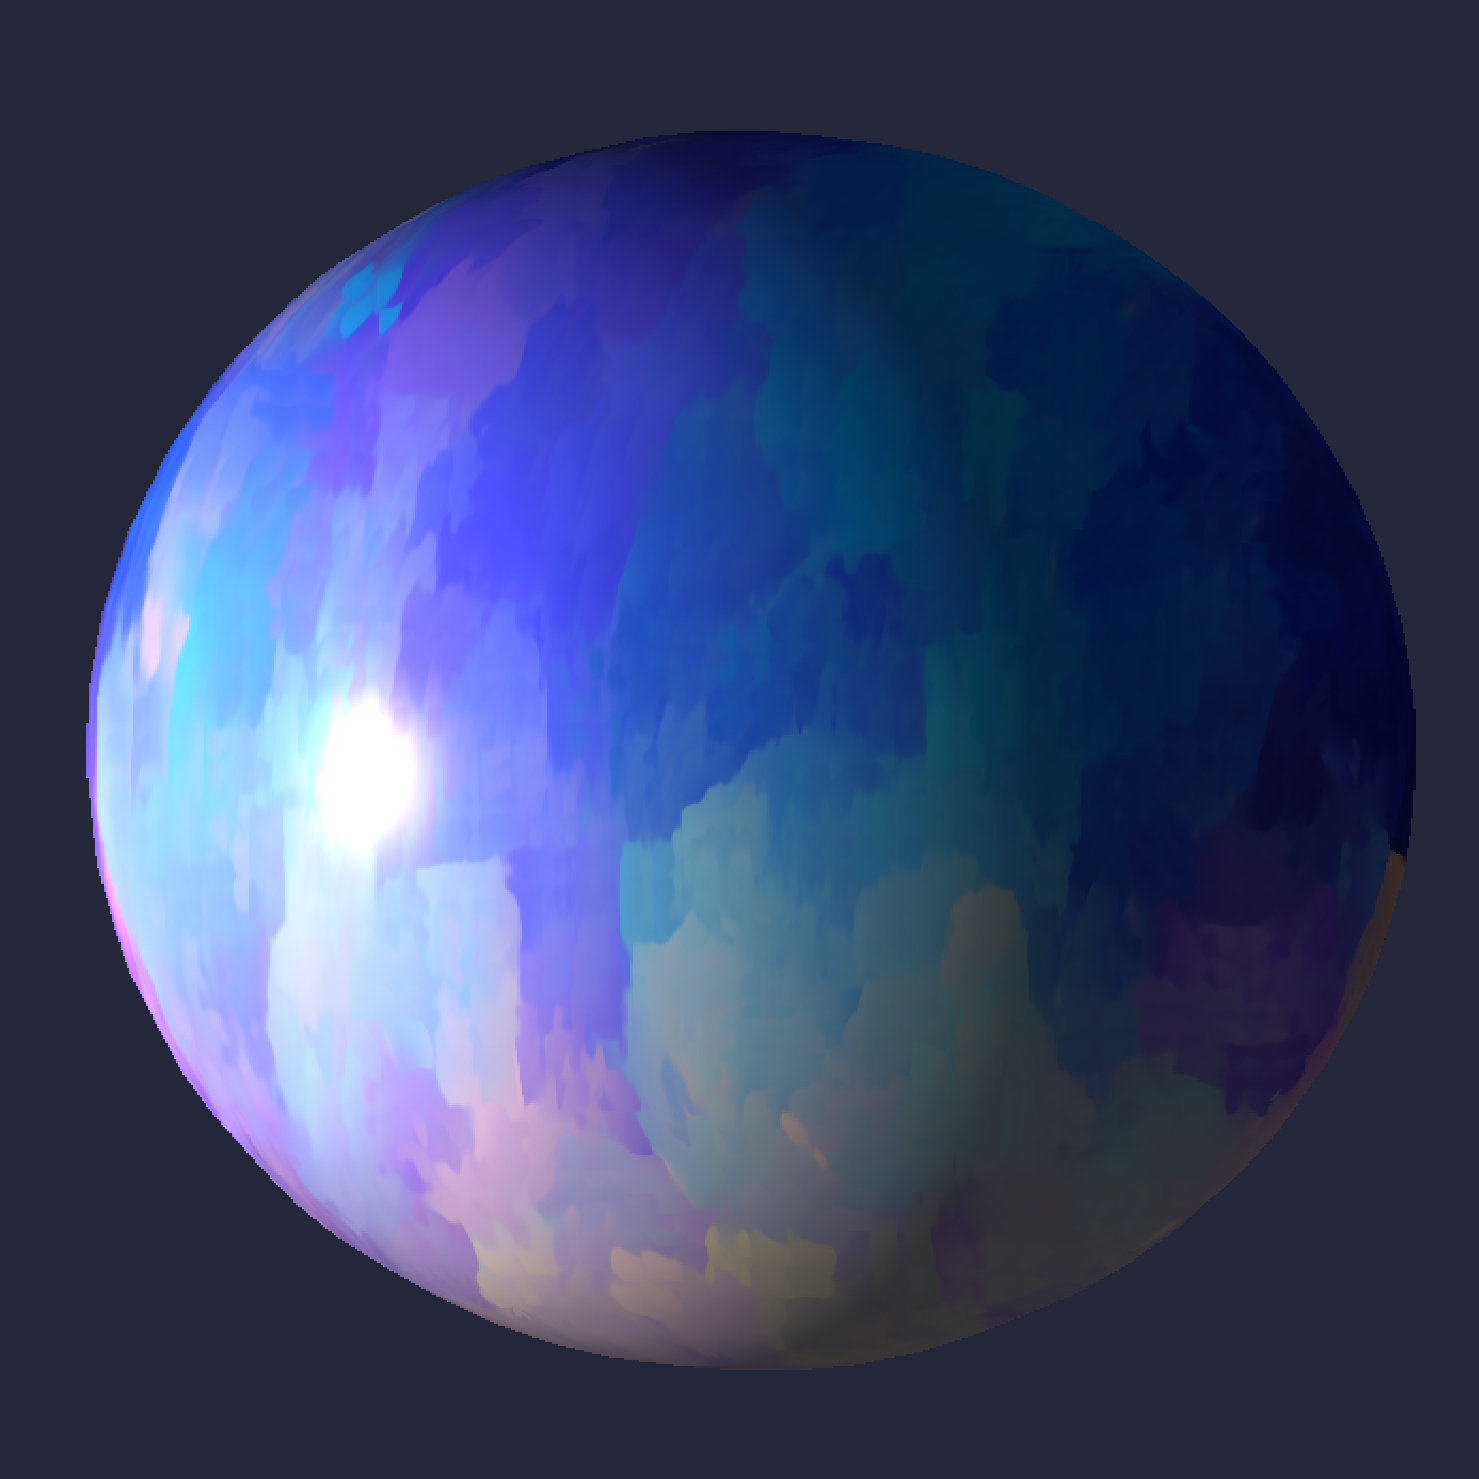
\includegraphics[width=0.85\linewidth]{abbildungen/hydra_capture_20260712_123807}
        \caption{Pre-Lit Kuwahara in Deferred-Uber}
        \label{fig:hydra_pre-lit}
    \end{subfigure}
    \hfill
% Rechtes Bild
    \begin{subfigure}[b]{0.49\textwidth}
        \centering
        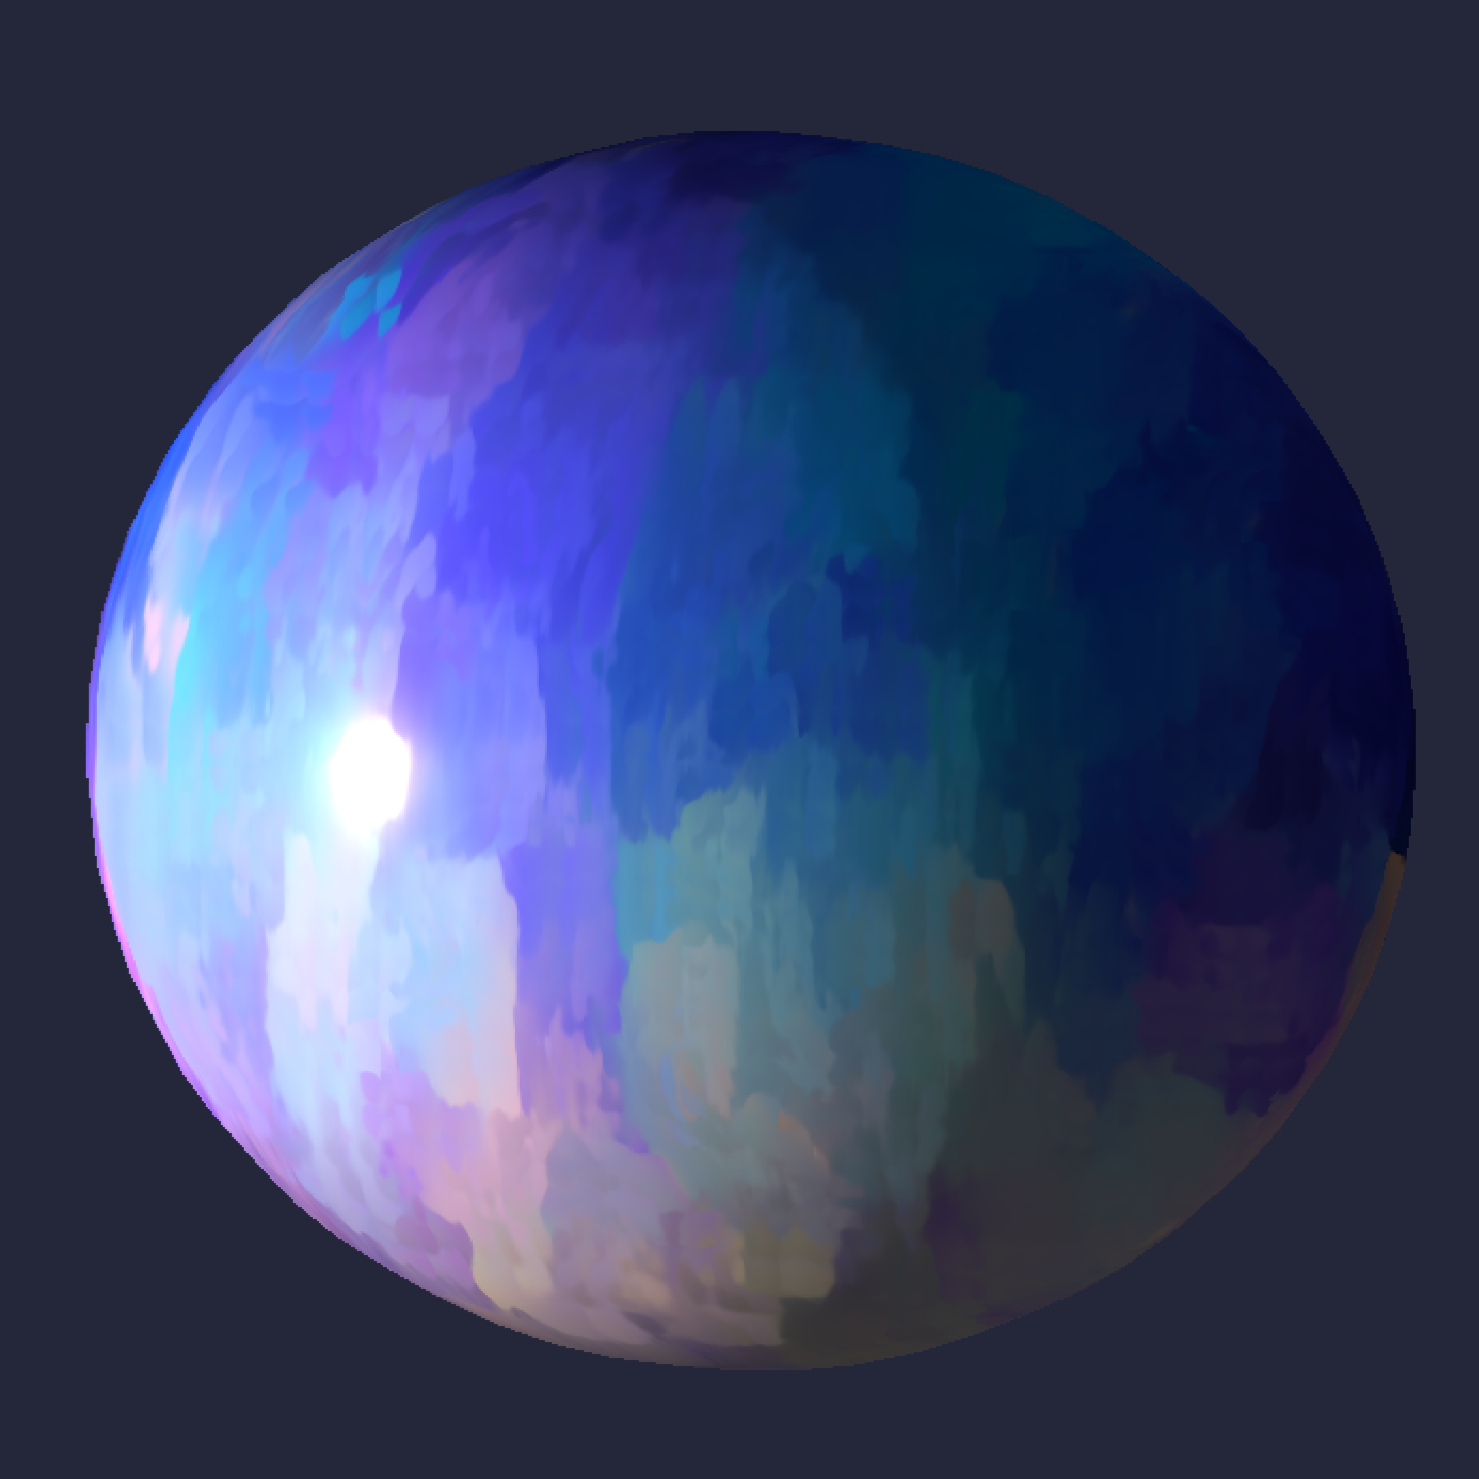
\includegraphics[width=0.85\linewidth]{abbildungen/hydra_capture_20260712_123817}
        \caption{Post-Lit Kuwahara in Deferred-Volume}
        \label{fig:hydra_post-lit}
    \end{subfigure}
    \caption{Visueller Vergleich von Pre-Lit und Post-Lit Kuwahara in HyDra-Framework.}
    \label{fig:040202_pre-post-lit_comparison}
\end{figure}

\subsection{Deferred-Volume Rendering Pipeline}
\label{subsec:040203_deferred_volume_pipeline}

% Einführung und Entscheidung.
Zusätzlich zur Deferred-Uber-Pipeline wurde im \ac{HyDra}-Framework eine weitere Deferred-Pipeline implementiert, um die
ebenfalls weit verbreiteten Multi-Pass-Rendering-Verfahren (bezogen auf den Lighting-Pass) zu repräsentieren und
vergleichend heranzuziehen.
Dieses Paradigma reflektiert den in der Praxis wesentlich verbreiteteren Ansatz in
Deferred-Pipelines~\cite[Folie~5]{lauritzenDeferredRenderingCurrent}, ohne dabei auf fortgeschrittene
Optimierungsverfahren zurückzugreifen.
Zu diesem Zweck wird die Deferred-Volume-Pipeline implementiert.
Deferred Rendering mit Light-Volumes zeichnet sich, wie in Kapitel~\ref{KapitelVolumes} dargelegt, durch das Zeichnen
von Proxy-Geometrien (hier in Form einer Kugel) um die entsprechenden Punktlichtquellen aus.
Der vorliegende Ansatz löst den in der Deferred-Uber-Pipeline verwendeten Uber-Shader in zwei ausgelagerte Pässe auf.
Dies erfolgt, indem die Beleuchtungslogik in isolierte, iterative Draw-Calls verpackt wird.

% Performance-Tease.
Die Charakteristische-Last der Deferred-Volume-Pipeline zeigt sich hier in einem anderen Bereich und
wird, durch das additive Blending der Light-Volumes, im Framebuffer in den \ac{ROP}s und in der \ac{VRAM}-Bandbreite
verortet~\cite[Folie~9]{lauritzenDeferredRenderingCurrent}[S.~676]{gregoryGameEngineArchitecture2018}.
Die genauen performancetechnischen Auswirkungen werden in der empirischen Evaluation in Kapitel~\ref{ch:05_evaluation}
(insbesondere in Abschnitt~\ref{subsec:050402_light_intensity_and_overlap_eval}) quantitativ analysiert.

% Banding.
Ein signifikanter architektonischer Unterschied zwischen der monolithischen Deferred-Uber-Pipeline und der
Deferred-Volume-Pipeline äußert sich in der Anfälligkeit für visuelle Quantisierungsartefakte (Color Banding) bei der
Verwendung von Bildformaten mit niedriger Bit-Tiefe (8-Bit pro Kanal) innerhalb der \ac{G-Buffer}.
In Ansätzen mit einem einzigen Lighting-Pass erfolgt die Akkumulation der Lichtbeiträge innerhalb einer Schleife auf
Treiberebene in lokalen \ac{GPU}-Registern mit nativer
32-Bit-Fließkommapräzision~\cite[Kap.~11.2.5.1, Abschn.~\textit{Shader Registers}]{gregoryGameEngineArchitecture2018}.
Im Gegensatz dazu entkoppelt die Deferred-Volume-Pipeline die Lichtberechnung in diskrete Pässe, deren
Ergebnisse mittels additiven Hardware-Blending (\textit{Blending Stage}) im Framebuffer aufsummiert werden.
Wird hierbei ein 8-Bit-Puffer verwendet, unterliegt das Zwischenergebnis nach der Evaluierung jedes
einzelnen Lichtvolumens einer fortlaufenden Quantisierung sowie einer harten Rundung auf den Wertebereich $[0, 1]$
(\textit{Clamping})~\cite[Kap.~4.1.7]{OpenGL33Core2010}.
Die wiederholte Rundung der Lichtbeiträge führt zu einer Akkumulation von Rundungsfehlern, die sich visuell
als stufenförmige Banding-Artefakte darstellen (siehe Abbildung~\ref{fig:hydra_banding_comparison}).
Diese Artefakte sind besonders in künstlerischen und abstrahierenden Effekten, wei sie im \ac{NPR} anwendung finden,
von Signifikanz (siehe Abbildung~\ref{fig:hydra_clamping_comparison}).
Die Deferred-Volume-Pipeline ist folglich zwingend auf \ac{HDR} mit mindestens 16-Bit-Fließkommapräzision zur
Kompensation dieses Präzisionsverlusts und Vermeidung von Farbsättigung (\textit{Clamping}) angewiesen.
Dieser Umstand erhöht die \ac{VRAM}-Belastung Deferred-Volume-Pipelines im Vergeblich zu den anderen Pipelines.

% Quantisierungsartefakte (Color Banding)
\begin{figure}[htbp]
    \centering
    \begin{subfigure}[b]{0.49\textwidth}
        \centering
        
\includegraphics[width=0.85\linewidth]{abbildungen/hydra_capture_20260430_153519}
        \caption{16-Bit Fließkommapräzision (HDR)}
        \label{fig:hydra_volume_hdr_gradient}
    \end{subfigure}
    \hfill
    \begin{subfigure}[b]{0.49\textwidth}
        \centering
        
\includegraphics[width=0.85\linewidth]{abbildungen/hydra_capture_20260430_153528}
        \caption{8-Bit Fixpunktpräzision (LDR)}
        \label{fig:hydra_volume_ldr_banding}
    \end{subfigure}
    \caption{Visueller Vergleich der Lichtakkumulation zur Isolation von Quantisierungsartefakten in
    Deferred-Volume-Pipeline in HyDra-Framework.}
    \label{fig:hydra_banding_comparison}
\end{figure}

% Sättigungsartefakte (Clamping)
\begin{figure}[htbp]
    \centering
    \begin{subfigure}[b]{0.49\textwidth}
        \centering
        
\includegraphics[width=0.85\linewidth]{abbildungen/hydra_capture_20260430_151409}
        \caption{Verlustfreie Akkumulation (16-Bit HDR)}
        \label{fig:hydra_kuwahara_hdr_correct}
    \end{subfigure}
    \hfill
    \begin{subfigure}[b]{0.49\textwidth}
        \centering
        
\includegraphics[width=0.85\linewidth]{abbildungen/hydra_capture_20260430_151418}
        \caption{Farbclamping und Posterisierung (8-Bit LDR)}
        \label{fig:hydra_kuwahara_ldr_clamping}
    \end{subfigure}
    \caption{Auswirkung des Framebuffer-Präzisionsformats auf die Integrität des Kuwahara-Filters in
    Deferred-Volume-Pipeline in HyDra-Framework.}
    \label{fig:hydra_clamping_comparison}
\end{figure}

% Post-Lit Vorteil
Im Gegensatz zur Deferred-Uber-Architektur bietet die Deferred-Volume-Architektur den Vorteil, dass Bildraumeffekte,
ohne den Zwang Pre-Lit-Verfahren anzuwenden, mit Post-Lit-Verfahren aufbereitet werden können
(vergleiche Abbildung~\ref{fig:040202_pre-post-lit_comparison}).
Für die spätere Performance-Analyse (siehe Kapitel~\ref{ch:05_evaluation}) ist jedoch zu bemerken, dass diese
Post-Lit-Evaluierungen mit einem leicht erhöhten algorithmischen Aufwand verbunden sind.
Dieser begründet sich im Resolve-Pass der Deferred-Volume-Pipeline durch die multiplen Texturzugriffe pro Kernel-Sample,
also konkret das simultane Abfragen von G-Buffer-Identitätsdaten und dem akkumulierten Lichtpuffer.
Im Pre-Lit-Verfahren der Deferred-Uber-Pipeline müssen dagegen nur die Albedo-Daten (Farbinformationen) der Nachbarpixel
ausgelesen werden.


\section{NPR-Payloads}
\label{sec:0403_npr_payloads}

% Einleitung und Auflistung.
Für die Evaluation der zugrunde liegenden Rendering-Pipelines werden im \ac{HyDra}-Framework neben einer Baseline
(Blinn-Phong-Shading) verschiedene \ac{NPR}-Effekte implementiert.
Im Folgenden werden die Charakteristika der verwendeten Stile sowie ihre grundlegende algorithmische Komplexität
erläutert, um sie für die in Kapitel 5 durchgeführten Evaluationen zu kontextualisieren.
Eine detaillierte Beschreibung der Implementierung wird in dieser Arbeit nicht vorgenommen, da für alle
\ac{NPR}-Effekte und das Baseline-Shading die jeweils etablierten Standardlösungen implementiert wurden.
Die implementierten Effekte fungieren demnach lediglich als reine Payloads (Lastgeneratoren) für die Evaluation der
selektiven Stilisierung unter Anwendung der verschiedenen Rendering-Verfahren.

Für das \ac{HyDra}-Framework sind die in Tabelle~\ref{tab:shading_effects} beschriebenen Effekte bzw.\ Stile verwendet
worden.

\begin{longtable}{@{} p{0.2\textwidth} p{0.4\textwidth} p{0.35\textwidth} @{}}
    \caption{Vergleich der verwendeten Shading-Effekte und NPR-Stile in HyDra-Framework.}
    \label{tab:shading_effects} \\
    \toprule
    \textbf{Effekt} & \textbf{Algorithmische Charakteristika} & \textbf{Semantische Charakteristika} \\
    \midrule
    \endfirsthead

    \multicolumn{3}{c}{{\tablename\ \thetable{} -- Fortsetzung}} \\
    \toprule
    \textbf{Effekt} & \textbf{Algorithmische Charakteristika} & \textbf{Semantische Charakteristika} \\
    \midrule
    \endhead

    \midrule
    \multicolumn{3}{r}{{Weiter auf der nächsten Seite...}} \\
    \endfoot

    \bottomrule
    \endlastfoot

    \textbf{Kuwahara}\newline \cites{kyprianidisImageVideoAbstraction2009}{papariArtisticEdgeCorner2007} &
    Iterative Kernel-Texture-Fetches in 4 Quadranten zur Varianz- und Mittelwertberechnung.
    Radiusabhängige Schleifen.
    & Erzeugt eine stilisierte, malerische Abstraktion (Painterly-Look) durch Homogenisierung lokaler Farbflächen
    (siehe Abb.~\ref{fig:040202_pre-post-lit_comparison}).\\
    \addlinespace

    \midrule

    \textbf{Toon}\newline \cite{lakeStylizedRenderingTechniques2000} &
    Dot-Products ($N \cdot L$) und Quantisierung (Banding) der diffusen Beleuchtung über Floor/Step-Funktionen.
    & Reduziert kontinuierliche Schattierungsverläufe auf diskrete Helligkeitsstufen; Charakteristisch für die Ästhetik
    klassischer Cel-Animationen (siehe Abb.~\ref{fig:040201_outline_comparison}). \\
    \addlinespace

    \midrule

    \textbf{Gooch}\newline \cite{goochNonphotorealisticLightingModel1998} &
    Lineare Interpolation zwischen definierten Cool- und Warm-Colors basierend auf dem Skalarprodukt ($N \cdot L$).
    & Verbessert die visuelle Wahrnehmung von Geometriedetails durch Temperaturkontraste; Vorrangig verwendet für
    technische Illustrationen (siehe Abb.~\ref{fig:gooch_example}). \\
    \addlinespace

    \midrule

    \textbf{Sobel}\newline \cite[Kap.~3.3]{saitoComprehensibleRendering3D1990} &
    Diskrete~$3\times3$ Kernel-Texture-Fetches auf Depth- und Normal-Buffern im \ac{G-Buffer} zur Gradienten- und
    Kantenerkennung.
    & Extrahiert und betont Geometrie- sowie Tiefendiskontinuitäten zur klaren visuellen Segmentierung von Objekten im
    Bildraum (siehe Abb.~\ref{fig:hydra_sobel-outlines}). \\
    \addlinespace

    \midrule

    \textbf{Inverted-Hull}\newline \cite[Kap.~15.2.2]{akenine-mollerRealtimeRendering2019} &
    Verschieben der Oberfläche entlang der Normalen bei gleichzeitiger Umkehrung der gerenderten Flächen.
    & Generiert eine konsistente, geschlossene Außenkontur im Objektraum durch das vergrößerte Rendern der maskierten
    Rückseiten (siehe Abb.~\ref{fig:hydra_inverted-hull}). \\
\end{longtable}

\begin{figure}[htbp]
    \centering
    
\includegraphics[width=0.85\linewidth]{abbildungen/hydra_capture_20260712_222142}
    \caption{Gooch-Shading in HyDra-Framework.}
    \label{fig:gooch_example}
\end{figure}

% Kanten-Bleeding
Ein inhärentes Problem der selektiven Kuwahara-Filterung in Deferred Pipelines äußert sich bei Objekten mit sehr
geringer projizierter Bildschirmfläche.
Da bei bildschirmbasierten Operatoren die Arbeit auf einer festen Pixel-Nachbarschaft erfolgt, kommt es bei einer
Verkleinerung des Objekts (z.\ B.\ durch zunehmende Kameraentfernung) oder an den Objekträndern zu einem Verlust oder
der inhaltlichen Verfälschung der notwendigen diskreten Abtastpunkte innerhalb der
Objektgrenzen~\cite[Abschn.~5]{kyprianidisImageVideoAbstraction2009}
(siehe Abb.~\ref{fig:npr_spatial_low_pixel_problem}).
Innerhalb des \ac{HyDra}-Frameworks werden zur Umgehung dieser Effekte jene Samples verworfen, deren \texttt{styleID}
nicht mit dem Zentrum übereinstimmt, um eine Verrechnung benachbarter Objekte mit unterschiedlicher Stilisierung zu
verhindern.
Diese werden durch einen konstanten Fallback-Wert in Form der unfiltrierten Basisfarbe des gezeichneten Pixels ersetzt
(vergleiche Listing~\ref{lst:kuwahara_optimization}).
Diese Modifikation dient der Gewährleistung einer stilistischen Parität des Kuwahara-Filters auch bei selektiver
Anwendung des Effektes.

\begin{figure}[htbp]
    \centering
    
\includegraphics[width=0.85\linewidth]{abbildungen/hydra_capture_20260524_103923}
    \caption{Kollabieren der selektiven Kuwahara-Bildraumfilterung bei weit entfernten und kleinen Geometrien in
    HyDra-Framework (vergrößerte Darstellung).}
    \label{fig:npr_spatial_low_pixel_problem}
\end{figure}

% Entropie Listing.
\begin{listing}[htbp]
    \begin{codeframe}
        \begin{minted}{glsl}
// Fetch neighbor's spatial and identity data
vec4 neighborNormalData = texture(gNormalTex, sampleUV);
int neighborStyleID = int(round(neighborNormalData.a * 255.0));
vec3 col;

// Validate Neighbor
if (neighborStyleID != styleID) {
    // Invalid: Clamp to the fully lit center pixel
    col = centerCol;
} else {
    // Valid: Sample actual neighbor lit color + ambient
    vec3 sampledLit = texture(litSceneTex, sampleUV).rgb;
    vec3 sampledAlbedo = texture(texture0, sampleUV).rgb;
    vec3 sampledAmbient = sampledAlbedo * ambientLightStrength;
    col = sampledLit + sampledAmbient;
}
        \end{minted}
    \end{codeframe}
    \caption{GLSL Code zur Optimierung von Kuwahara-Filter-Sampling zur Mitigierung von Kanten-Bleeding Effekten in der
    Deferred-Volume-Pipeline in HyDra-Framework.}
    \label{lst:kuwahara_optimization}
\end{listing}

% Mathematisch
Wie~\textcite[Abschn.~II-B]{papariArtisticEdgeCorner2007} darlegen, leidet die klassische Kuwahara-Filterstruktur unter
einer inhärenten mathematischen Instabilität, sobald mehrere Subregionen identische Standardabweichungen aufweisen.
Bei kleinen oder weit entfernten Geometrien wird dieser Zustand erzwungen.
Da das Objekt nicht mehr genügend Pixel besitzt, um den Kernel zu füllen, dominieren die konstanten Fallback-Werte der
Identitäts-Maskierung die Quadranten.
Die Varianz der abgetasteten Nachbarpixel sinkt hierbei gegen null, wodurch der Algorithmus die mathematische Basis
verliert, eine eindeutige Region zu isolieren.


\section{Telemetrie \& Benchmark-Orchestrierung}
\label{sec:0404_telemetry_and_benchmark_orchestrator}

% Einleitung.
Nachdem die architektonischen Limitationen und Charakteristika der implementierten Rendering-Pipelines dargelegt wurden,
müssen für die detaillierten Performancemessungen in Kapitel~\ref{ch:05_evaluation} die verwendeten Telemetrie- und
Benchmark-Orchestrierungsmodule definiert werden, um den Versuchsmethodik und produzierten Ergebnisse zu
kontextualisieren.

\subsection{Szenen- \& Zustandsparität}
\label{subsec:040401_scene_and_state_parity}

% Einleitung.
Ein objektiver Vergleich und die Belastbarkeit empirischer Performancedaten der verschiedenen Rendering-Pipelines in der
Echtzeitgrafik erfordern die technische Garantie, dass jede Pipeline pro Frame exakt denselben Workload verarbeitet.
Wenn eine Architektur durch abweichende Frustum-Culling-Berechnungen oder abweichende Licht-Allokationen weniger Last
auf die \ac{GPU} überträgt, verlieren die Untersuchungen ihre Validität.

% Engine State.
Die Systemarchitektur des \ac{HyDra}-Frameworks basiert zu diesem Zweck auf einem zentralen \texttt{EngineState}
(vergleiche Listing~\ref{lst:Engine_State}).
Dieser geteilte Zustand fungiert als zentrale Quelle für das Verhalten und den Gesamtaufbau der Szene sowie der
verwendeten Rendering-Pipelines der gesamten Laufzeitumgebung.
Das \texttt{BenchmarkOrchestrator}-Modul wendet vor dem Start und während jeder Testreihe sämtliche Variablenänderungen
(wie Instanzenanzahl, Detailgrad oder Filter-Radien) exakt einmal auf den globalen Zustand an und variiert im
Testverlauf lediglich die untersuchte unabhängige Variable (vergleiche Tab.~\ref{tab:independent_vars}).
Wie in Kapitel~\ref{subsec:040102_scene_management} dargelegt nutzen alle untersuchten Rendering-Pipelines über die
Variablen des \texttt{EngineState}s hinaus die gleiche Logik bezüglich Sichtbarkeitsprüfung und Geometrieverwaltung
unter Verwendung des \texttt{SceneManager}-Moduls.
Die Entkopplung von Datenhaltung und Render-Ausführung zielt demnach darauf ab, Divergenzen auf Szenen- und
Geometrie-Verwaltungsebene zwischen den verschiedenen Pipelines zu vermeiden.

% Engine State Listing.
\begin{listing}[htbp]
    \begin{codeframe}
        \begin{minted}{cpp}
// Architectural Rendering Paths
enum class RenderPath { DeferredUber, DeferredVolume, Forward };

// Centralized state container for the current frame
struct EngineState {
    RenderPath activeRenderPath = RenderPath::Forward;

    // Core Metrics
    bool use16BitHDR           = Config::DefaultState::Use16BitHDR;
    int activeObstacleCount    = Config::DefaultState::ActiveObstacleCount;
    int activeLightCount       = Config::DefaultState::ActiveLightCount;
    float lightIntensity       = Config::EngineSettings::LightIntensity;
    float ambientLightStrength = Config::EngineSettings::AmbientLightStrength;
    int renderWidth            = Config::EngineSettings::ScreenWidth;
    int renderHeight           = Config::EngineSettings::ScreenHeight;

    // NPR Toggles
    bool enableOutlines = Config::DefaultState::EnableOutlines;
    bool enableKuwahara = Config::DefaultState::EnableKuwahara;
    bool enableGooch    = Config::DefaultState::EnableGooch;
    bool enableToon     = Config::DefaultState::EnableToon;

    // Spatial & Stylistic Modifiers
    int kuwaharaRadius       = Config::DefaultState::KuwaharaRadius;
    float kuwaharaIntensity  = Config::DefaultState::KuwaharaIntensity;
    float objectSphereRadius = Config::DefaultState::ObjectSphereRadius;
    int currentLodIndex      = Config::DefaultState::CurrentLodIndex;

    // Architecture & Distribution Flags
    bool useClusteredStyles  = Config::DefaultState::UseClusteredStyles;
    bool useLightSingularity = Config::DefaultState::UseLightSingularity;
    bool useNprRoom          = Config::DefaultState::UseNprRoom;
    bool renderFloor         = Config::DefaultState::RenderFloor;

    // System Flags
    bool requestScreenshot = false;
};
        \end{minted}
    \end{codeframe}
    \caption{C++ Code zur Beschreibung des Zentralen Engine-Zustands in HyDra-Framework}
    \label{lst:Engine_State}
\end{listing}

\subsection{Asynchrone Hardware-Telemetrie}
\label{subsec:040401_async_hardware_telemetry}

% Einleitung
Die Erfassung von Ausführungszeiten auf der Host-Seite (\ac{CPU}) ist für die Bewertung der reinen
\ac{GPU}-Leistung unzureichend, da moderne Grafiktreiber hochgradig asynchron
arbeiten~\cite[S.~1005]{akenine-mollerRealtimeRendering2019}.
Die \ac{CPU} sendet Render-Kommandos an eine Warteschlange und setzt die Ausführung unmittelbar fort, noch bevor die
\ac{GPU} das erste Polygon
verarbeitet~\cite[Abschn.~\textit{The logical pipeline} 1-2]{pixeljetstreamPixelJetStream2015}.

% Verfahren.
Das \ac{HyDra}-Framework injiziert über \texttt{glQueryCounter} asynchrone Zeitstempel direkt in den
\ac{GPU}-Befehlsstrom.
Diese \textit{OpenGL Query Objects} ermöglichen eine hardwareseitige Zeiterfassung, um die Ausführungsdauer der
einzelnen Render-Pässe isoliert zu messen~\cite[Kap.~2.14]{OpenGL33Core2010}.
Da das unmittelbare Auslesen dieser Markierungen im selben Frame einen kritischen Pipeline-Stall erzeugen
würde~\cite[S.~794]{akenine-mollerRealtimeRendering2019},
implementiert die \texttt{GpuProfiler}-Klasse ein asynchrones Ring-Buffer-Verfahren~\cite[Kap.~34.2.5]{OpenGLInsights},
um die Grafikkarten-Abläufe im Normalfall nicht zu blockieren (\textit{Non-Blocking}).
Durch die strikte Begrenzung der maximal im Flug befindlichen Frame-Abfragen
auf~\texttt{GpuProfiler::MAX\_IN\_FLIGHT = 16} verhindert der \texttt{BenchmarkOrchestrator} zudem bei hoher
\ac{GPU}-Auslastung ein Überschreiben noch nicht ausgelesener Hardware-Abfragen der \ac{GPU} durch die \ac{CPU}.
Der kontrollierte \textquote{Notfall-Stall} stoppt die \ac{CPU}-Befehlsübertragung und stellt somit sicher, dass jeder
gerenderte Frame ohne Datenverlust lückenlos und chronologisch in die Telemetrie einfließt
(vergleiche Listing~\ref{lst:orchestrator_stall}).

% Orchestrator Listing:
\begin{listing}[htbp]
    \begin{codeframe}
        \begin{minted}{cpp}
// Queue up the raw CPU metrics for this frame
pendingFrames.push(FrameRecord{...});

// Process resolved frames
while (!pendingFrames.empty()) {
    const auto &[...] = pendingFrames.front();
    const bool isDeferred = (recActiveRenderPath != RenderPath::Forward);

    // Check if hardware queries are naturally ready
    const bool geomReady       = !isDeferred || geomProfiler.IsOldestReady();
    const bool lightReady      = lightProfiler.IsOldestReady();
    const bool masterReady     = masterGpuProfiler.IsOldestReady();
    const bool allQueriesReady = (geomReady && lightReady && masterReady);
    const bool emergencyStallRequired =
        (pendingFrames.size() >= GpuProfiler::MAX_IN_FLIGHT);

    // Wait for all profilers to report, or force wait to clear capacity
    if (allQueriesReady || emergencyStallRequired) {
        double geomMs = 0.0, lightMs = 0.0, totalGpuMs = 0.0;

        // Pass 'forceWait' down to TryGetOldestResult so thread blocks and waits for the OpenGL queries to resolve before extracting
        if (isDeferred)
            geomProfiler.TryGetOldestResult(geomMs, emergencyStallRequired);
        lightProfiler.TryGetOldestResult(lightMs, emergencyStallRequired);
        masterGpuProfiler.TryGetOldestResult(totalGpuMs, emergencyStallRequired);

        telemetryWriter.AppendRow(...);
        pendingFrames.pop();
    } else {
        break; // GPU data for the oldest frame is not ready; Pause writes
    }
}
        \end{minted}
    \end{codeframe}
    \caption{C++ Code zu Ring-Buffer und Notfall-Stall Verfahren während der Benchmark-Orchestrierung in
    HyDra-Framework}
    \label{lst:orchestrator_stall}
\end{listing}

